\section{Scheibe}
    \subsection{Definition}
        \begin{wrapfigure}[7]{r}{0.5\linewidth}
            \vspace{-5mm}
            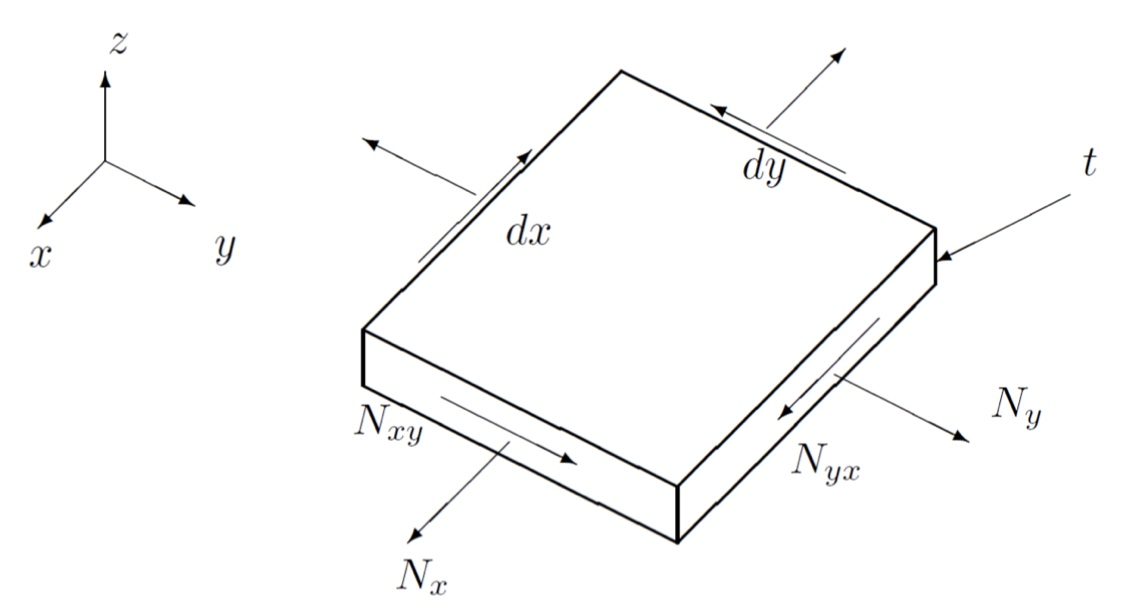
\includegraphics[width=\linewidth]{03/Scheibe}
        \end{wrapfigure}
        \textbf{Scheibenelement:} Dünnwandige Struktur mit Belastung in der Ebene. Äussere Kräfte dargestellt durch $N_x,N_y,N_{xy},N_{yx}$: Kräfte pro Längeneinheit ($\rightarrow$ Spannungen $\sigma_{xx},\sigma_{yy},\tau_{xy}$ über Dicke t integriert).
    
    \subsection{Annahmen}
        \begin{enumerate}[noitemsep]
            \item \textbf{Ebener Spannungszustand} ($\sigma_{zz},\tau_{xz},\tau_{yz}=0$)
            \item Übrige Spannungskomponenten sind konstant verteilt in z-Richtung (homogene Spannungsverteilung)
            \item Keine Volumenkräfte
            \item \textbf{Spannungsansatz} (GGB erfüllt)
        \end{enumerate}
        %\vspace{-1mm}
        1, 2: Vernünftig, weil planare Dimensionen $\gg$ t \& keine Biegung. GGB reduziert sich zu: $\displaystyle\sigma_{xx,x} + \tau_{xy,y}=0$; $\sigma_{yy,y} + \tau_{xy,x}=0$
        $\rightarrow$Definiere $F(x,y)$ (ayrische Spannungsfkt) mit:\\ $\sigma_{xx}=F_{,yy}$; $\sigma_{yy}=F_{,xx}$; $\tau_{xy}=-F_{,xy}$. 
        \\Aus Kompatibilitätsbedingung:\\ $\varepsilon_{xx,yy}+\varepsilon_{yy,xx}=2\varepsilon_{xy,xy} \rightarrow \Delta\Delta F=0$.
        \\Funktion F(x,y) so wählen, damit RB erfüllt.
\columnbreak    
    \subsection{Scheibe mit Loch}
    \vspace{-0.5mm}
        \begin{center}
            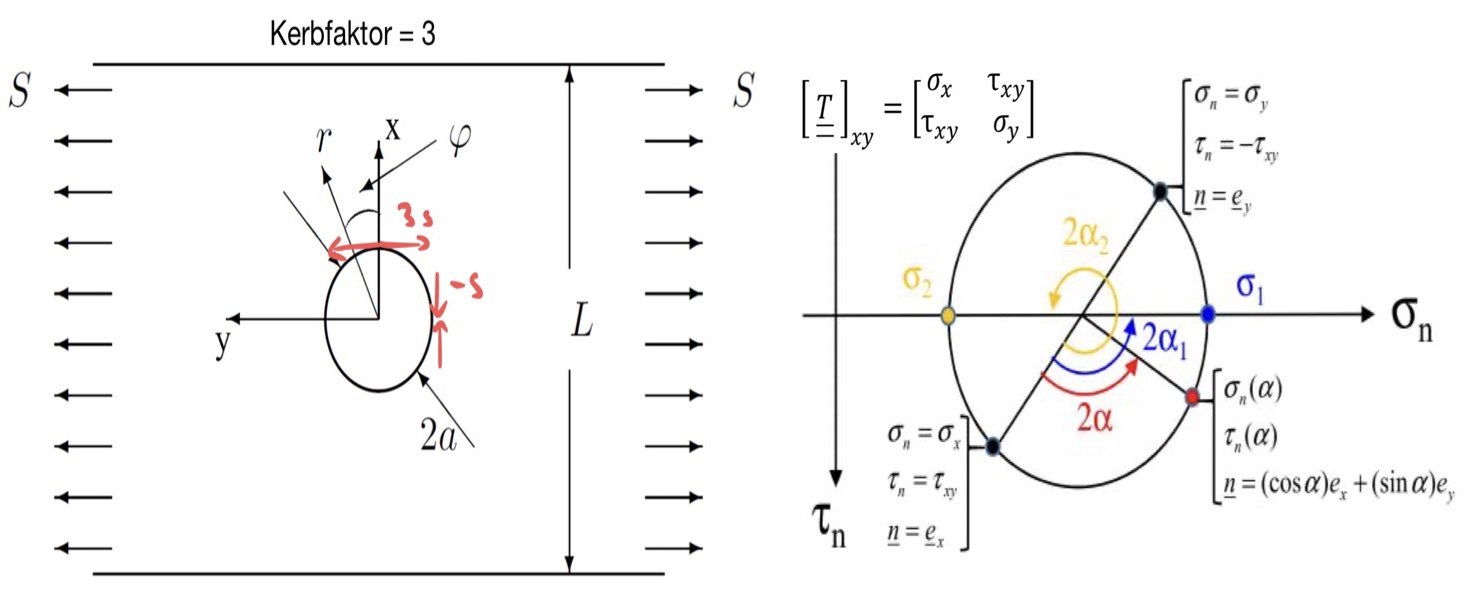
\includegraphics[width=\linewidth, height=25mm]{images/03/mohr_and_loch.jpeg}
        \end{center}
        \vspace{-3mm}
        \begin{itemize}
            \item Lochradius a $\ll$ L
            \item Belastung durch uniforme, einachsige Spannung S in grosser Entfernung vom Loch
            \item Spannungsfreie Rissflanken ($r = a; \forall\varphi\in\mathbb{R} $): $\sigma_{rr}=0, \tau_{r\varphi}=0$
        \end{itemize}
        \vspace{-2mm}
        \textbf{Superposition} von mehreren Spannungen \& Spannungsrichtungen möglich. Bei Schubspannungen in Hauptspannungen umwandlen (Mohrscher Kreis).
    \subsection{Scheibe mit Riss}
        Spannungsfreie Rissflanken ($\forall r, \varphi=\pm\pi$): $\sigma_{\varphi\varphi}=0, \tau_{r\varphi}=0$
        \begin{center}
            \vspace{-2mm}
            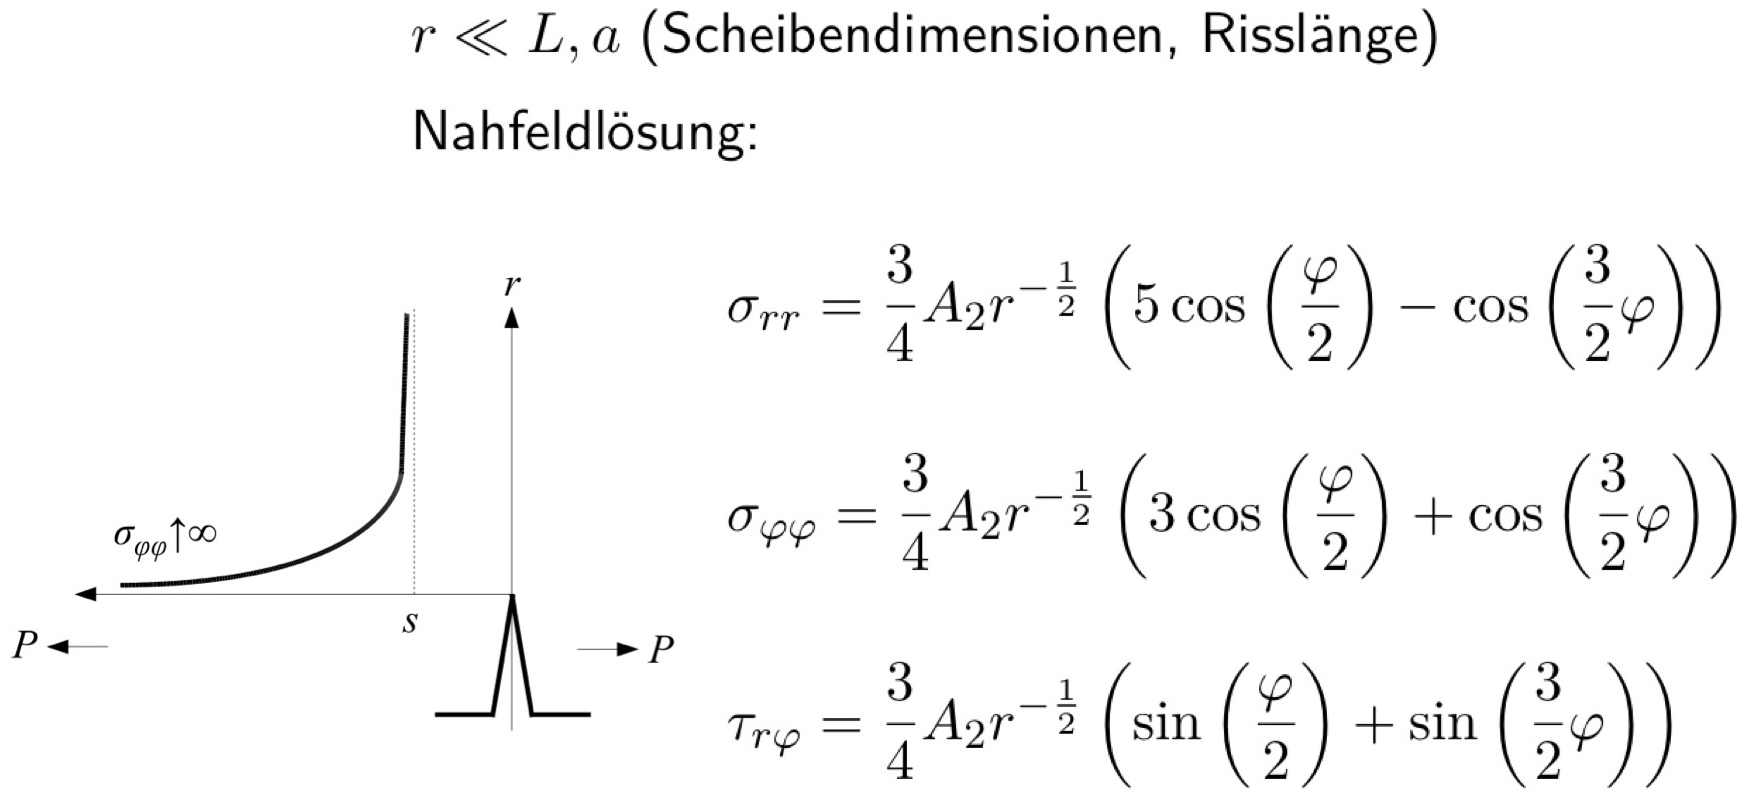
\includegraphics[width=75mm, height= 25mm]{03/Scheiberiss}
        \end{center}